\section{Approximation. Interpolation problem. Polynomial interpolation. Hermitian interpolation. Splines. Bézier curves and splines.}
{\hspace*{0.75cm} \begin{tikzpicture}[x=0.75pt,y=0.75pt,yscale=-1,xscale=1]
        %uncomment if require: \path (0,251); %set diagram left start at 0, and has height of 251
        
        %Straight Lines [id:da23080159581369686] 
        \draw [line width=1.5]    (145.3,227.02) -- (146.07,22.11) ;
        \draw [shift={(146.09,18.11)}, rotate = 90.22] [fill={rgb, 255:red, 0; green, 0; blue, 0 }  ][line width=0.08]  [draw opacity=0] (9.36,-2.34) -- (0,0) -- (9.36,2.34) -- cycle    ;
        %Straight Lines [id:da029066329694802384] 
        \draw [line width=1.5]    (105.65,207.98) -- (337.61,208.24) ;
        \draw [shift={(341.61,208.24)}, rotate = 180.06] [fill={rgb, 255:red, 0; green, 0; blue, 0 }  ][line width=0.08]  [draw opacity=0] (9.36,-2.34) -- (0,0) -- (9.36,2.34) -- cycle    ;
        %Curve Lines [id:da46449697572183446] 
        \draw [line width=1.5]    (155.6,201.29) .. controls (156.39,192.94) and (159.03,195.2) .. (182.11,123.43) .. controls (218.42,26.57) and (248.89,302.88) .. (335.23,122.47) ;
        %Shape: Ellipse [id:dp5533295702056344] 
        \draw  [fill={rgb, 255:red, 13; green, 13; blue, 13 }  ,fill opacity=1 ] (155.23,191.21) .. controls (155.23,188.99) and (157.09,187.19) .. (159.39,187.19) .. controls (161.69,187.19) and (163.55,188.99) .. (163.55,191.21) .. controls (163.55,193.43) and (161.69,195.23) .. (159.39,195.23) .. controls (157.09,195.23) and (155.23,193.43) .. (155.23,191.21) -- cycle ;
        %Shape: Ellipse [id:dp11622378818956114] 
        \draw  [fill={rgb, 255:red, 13; green, 13; blue, 13 }  ,fill opacity=1 ] (178.18,123.43) .. controls (178.18,121.21) and (180.04,119.41) .. (182.34,119.41) .. controls (184.64,119.41) and (186.5,121.21) .. (186.5,123.43) .. controls (186.5,125.65) and (184.64,127.45) .. (182.34,127.45) .. controls (180.04,127.45) and (178.18,125.65) .. (178.18,123.43) -- cycle ;
        %Shape: Ellipse [id:dp8604322146340477] 
        \draw  [fill={rgb, 255:red, 13; green, 13; blue, 13 }  ,fill opacity=1 ] (261.29,181.1) .. controls (261.29,178.88) and (263.15,177.08) .. (265.45,177.08) .. controls (267.74,177.08) and (269.61,178.88) .. (269.61,181.1) .. controls (269.61,183.33) and (267.74,185.13) .. (265.45,185.13) .. controls (263.15,185.13) and (261.29,183.33) .. (261.29,181.1) -- cycle ;
        %Shape: Ellipse [id:dp6476197024831782] 
        \draw  [fill={rgb, 255:red, 13; green, 13; blue, 13 }  ,fill opacity=1 ] (311.29,158.63) .. controls (311.29,156.4) and (313.16,154.6) .. (315.45,154.6) .. controls (317.75,154.6) and (319.61,156.4) .. (319.61,158.63) .. controls (319.61,160.85) and (317.75,162.65) .. (315.45,162.65) .. controls (313.16,162.65) and (311.29,160.85) .. (311.29,158.63) -- cycle ;
        %Straight Lines [id:da006280100300212643] 
        \draw [line width=1.5]    (531.78,226.97) -- (532.55,22.07) ;
        \draw [shift={(532.57,18.07)}, rotate = 90.22] [fill={rgb, 255:red, 0; green, 0; blue, 0 }  ][line width=0.08]  [draw opacity=0] (9.36,-2.34) -- (0,0) -- (9.36,2.34) -- cycle    ;
        %Straight Lines [id:da35076475417958886] 
        \draw [line width=1.5]    (492.13,207.94) -- (724.1,208.2) ;
        \draw [shift={(728.1,208.2)}, rotate = 180.06] [fill={rgb, 255:red, 0; green, 0; blue, 0 }  ][line width=0.08]  [draw opacity=0] (9.36,-2.34) -- (0,0) -- (9.36,2.34) -- cycle    ;
        %Shape: Ellipse [id:dp7804449233013961] 
        \draw  [fill={rgb, 255:red, 13; green, 13; blue, 13 }  ,fill opacity=1 ] (541.71,191.17) .. controls (541.71,188.94) and (543.57,187.14) .. (545.87,187.14) .. controls (548.17,187.14) and (550.03,188.94) .. (550.03,191.17) .. controls (550.03,193.39) and (548.17,195.19) .. (545.87,195.19) .. controls (543.57,195.19) and (541.71,193.39) .. (541.71,191.17) -- cycle ;
        %Shape: Ellipse [id:dp8399759569275331] 
        \draw  [fill={rgb, 255:red, 13; green, 13; blue, 13 }  ,fill opacity=1 ] (564.66,123.39) .. controls (564.66,121.16) and (566.52,119.36) .. (568.82,119.36) .. controls (571.12,119.36) and (572.98,121.16) .. (572.98,123.39) .. controls (572.98,125.61) and (571.12,127.41) .. (568.82,127.41) .. controls (566.52,127.41) and (564.66,125.61) .. (564.66,123.39) -- cycle ;
        %Shape: Ellipse [id:dp6967929166905409] 
        \draw  [fill={rgb, 255:red, 13; green, 13; blue, 13 }  ,fill opacity=1 ] (647.77,181.06) .. controls (647.77,178.84) and (649.63,177.04) .. (651.93,177.04) .. controls (654.22,177.04) and (656.09,178.84) .. (656.09,181.06) .. controls (656.09,183.28) and (654.22,185.09) .. (651.93,185.09) .. controls (649.63,185.09) and (647.77,183.28) .. (647.77,181.06) -- cycle ;
        %Shape: Ellipse [id:dp40286398040829696] 
        \draw  [fill={rgb, 255:red, 13; green, 13; blue, 13 }  ,fill opacity=1 ] (696.85,158.81) .. controls (696.85,156.59) and (698.71,154.78) .. (701.01,154.78) .. controls (703.3,154.78) and (705.17,156.59) .. (705.17,158.81) .. controls (705.17,161.03) and (703.3,162.83) .. (701.01,162.83) .. controls (698.71,162.83) and (696.85,161.03) .. (696.85,158.81) -- cycle ;
        %Curve Lines [id:da03032373857171078] 
        \draw [line width=1.5]  [dash pattern={on 1.69pt off 2.76pt}]  (138.14,169.09) .. controls (194.45,123.49) and (208.91,190.76) .. (265.22,145.16) .. controls (321.53,99.55) and (311.3,178.72) .. (346.49,140.72) ;
        %Curve Lines [id:da3945435615785029] 
        \draw [line width=1.5]    (542.32,201.25) .. controls (543.1,192.89) and (545.75,195.16) .. (568.82,123.39)(568.82,123.62) .. controls (605.14,26.76) and (635.6,302.83) .. (721.95,122.43) ;
        %Straight Lines [id:da6086554480503785] 
        \draw    (215.48,115.26) -- (221.06,93.97) ;
        %Straight Lines [id:da8312721119253743] 
        \draw    (1844,60) -- (1881.35,60) ;
        %Straight Lines [id:da6503699190659245] 
        \draw    (220.17,93.97) -- (260.19,93.98) ;
        %Straight Lines [id:da20940998884743434] 
        \draw    (285.17,130.46) -- (290.75,109.18) ;
        %Straight Lines [id:da5778528222852668] 
        \draw    (289.86,109.18) -- (369.3,109.18) ;
        %Straight Lines [id:da8927628943439354] 
        \draw  [dash pattern={on 2.25pt off 2.25pt on 2.25pt off 2.25pt}]  (568.82,123.62) -- (532.18,123.62) ;
        %Straight Lines [id:da8738872036751961] 
        \draw  [dash pattern={on 2.25pt off 2.25pt on 2.25pt off 2.25pt}]  (568.82,123.62) -- (567.76,207.83) ;
        %Straight Lines [id:da5868919836287383] 
        \draw  [dash pattern={on 2.25pt off 2.25pt on 2.25pt off 2.25pt}]  (545.87,191.17) -- (531.72,191.17) ;
        %Straight Lines [id:da25549069412078107] 
        \draw  [dash pattern={on 2.25pt off 2.25pt on 2.25pt off 2.25pt}]  (545.8,206.44) -- (545.87,191.17) ;
        %Straight Lines [id:da8522583894532492] 
        \draw  [dash pattern={on 2.25pt off 2.25pt on 2.25pt off 2.25pt}]  (651.93,180.63) -- (532.61,180.65) ;
        %Straight Lines [id:da0910754969790295] 
        \draw  [dash pattern={on 2.25pt off 2.25pt on 2.25pt off 2.25pt}]  (651.74,207.57) -- (651.93,181.06) ;
        %Straight Lines [id:da22854306729915708] 
        \draw  [dash pattern={on 2.25pt off 2.25pt on 2.25pt off 2.25pt}]  (701.01,158.81) -- (531.8,158.81) ;
        %Straight Lines [id:da5253855474936553] 
        \draw  [dash pattern={on 2.25pt off 2.25pt on 2.25pt off 2.25pt}]  (701.01,207.57) -- (701.01,158.81) ;
        
        % Text Node
        \draw (330.03,210.01) node [anchor=north west][inner sep=0.75pt]  [font=\footnotesize] [align=left] {$\displaystyle x$};
        % Text Node
        \draw (148.09,20.91) node [anchor=north west][inner sep=0.75pt]  [font=\footnotesize] [align=left] {$\displaystyle f( x)$};
        % Text Node
        \draw (715.51,208.97) node [anchor=north west][inner sep=0.75pt]  [font=\footnotesize] [align=left] {$\displaystyle x$};
        % Text Node
        \draw (534.57,20.87) node [anchor=north west][inner sep=0.75pt]  [font=\footnotesize] [align=left] {$\displaystyle f( x)$};
        % Text Node
        \draw (183.56,227.16) node [anchor=north west][inner sep=0.75pt]   [align=left] {Approximation};
        % Text Node
        \draw (570,227.16) node [anchor=north west][inner sep=0.75pt]   [align=left] {Interpolation};
        % Text Node
        \draw (222.32,82.15) node [anchor=north west][inner sep=0.75pt]  [font=\scriptsize] [align=left] {unknown};
        % Text Node
        \draw (291.16,97.36) node [anchor=north west][inner sep=0.75pt]  [font=\scriptsize] [align=left] {simple function};
        % Text Node
        \draw (541.17,210.8) node [anchor=north west][inner sep=0.75pt]  [font=\scriptsize] [align=left] {$\displaystyle x_{0}$};
        % Text Node
        \draw (564.99,210.8) node [anchor=north west][inner sep=0.75pt]  [font=\scriptsize] [align=left] {$\displaystyle x_{1}$};
        % Text Node
        \draw (650.16,210.8) node [anchor=north west][inner sep=0.75pt]  [font=\scriptsize] [align=left] {$\displaystyle x_{2}$};
        % Text Node
        \draw (699.08,210.8) node [anchor=north west][inner sep=0.75pt]  [font=\scriptsize] [align=left] {$\displaystyle x_{n}$};
        % Text Node
        \draw (519.65,185.53) node [anchor=north west][inner sep=0.75pt]  [font=\scriptsize] [align=left] {$\displaystyle y_{0}$};
        % Text Node
        \draw (519.65,173.89) node [anchor=north west][inner sep=0.75pt]  [font=\scriptsize] [align=left] {$\displaystyle y_{2}$};
        % Text Node
        \draw (519.65,151.61) node [anchor=north west][inner sep=0.75pt]  [font=\scriptsize] [align=left] {$\displaystyle y_{n}$};
        % Text Node
        \draw (519.65,116.64) node [anchor=north west][inner sep=0.75pt]  [font=\scriptsize] [align=left] {$\displaystyle y_{1}$};  
\end{tikzpicture}} \vspace*{-2cm}

\subsection*{Polynomial interpolation}
\subsubsection*{Classical problem of polynomial interpolation}
\underline{Problem}: Suppose some function $f(x) = a_0 + a_1x + a_2x^2 + \ldots + a_{n-1}x^{n-1} + a_{n} x^n$ is a polynomial of degree $\leq n$. Given the values of function $f(x)$:
\[
    \left\{ \begin{array}{c}
        f(x_0) = y_0, \\
        \ldots \\
        f(x_n) = y_n
    \end{array}\right.  
\]
Recover $f(x)$ is our goal. That is the main problem to find a vector $\vec{a} = \begin{bmatrix}
    a_0 & \ldots & a_n
\end{bmatrix}^\intercal = ?$
\vspace*{0.5cm}

{\large CRAMER,}{\large 1750}
\begin{wrapfigure}[6]{l}{0.45\columnwidth}
    \tikzset {_q6agbwvup/.code = {\pgfsetadditionalshadetransform{ \pgftransformshift{\pgfpoint{0 bp } { 0 bp }  }  \pgftransformscale{1 }  }}}
    \pgfdeclareradialshading{_q1fpvf47i}{\pgfpoint{0bp}{0bp}}{rgb(0bp)=(1,1,0);
    rgb(4.463268859045846bp)=(1,1,0);
    rgb(22.85699793270656bp)=(1,0,0);
    rgb(25bp)=(1,0,0);
    rgb(400bp)=(1,0,0)}
    
    \hspace*{0.75cm} 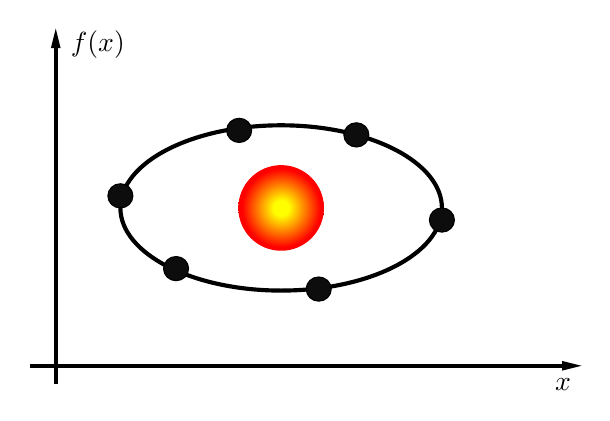
\begin{tikzpicture}[x=0.75pt,y=0.75pt,yscale=-1,xscale=1]
        %uncomment if require: \path (0,238); %set diagram left start at 0, and has height of 238
        
        %Straight Lines [id:da8941587014029553] 
        \draw [line width=1.5]    (144.18,201.47) -- (144.18,34.26) ;
        \draw [shift={(144.18,30.26)}, rotate = 90] [fill={rgb, 255:red, 0; green, 0; blue, 0 }  ][line width=0.08]  [draw opacity=0] (9.36,-2.34) -- (0,0) -- (9.36,2.34) -- cycle    ;
        %Straight Lines [id:da45851067481725116] 
        \draw [line width=1.5]    (131.65,192.73) -- (393.49,192.73) ;
        \draw [shift={(397.49,192.73)}, rotate = 180] [fill={rgb, 255:red, 0; green, 0; blue, 0 }  ][line width=0.08]  [draw opacity=0] (9.36,-2.34) -- (0,0) -- (9.36,2.34) -- cycle    ;
        %Shape: Ellipse [id:dp3419509937264853] 
        \draw  [line width=1.5]  (175.32,116.67) .. controls (175.32,94.68) and (209.99,76.86) .. (252.77,76.86) .. controls (295.55,76.86) and (330.23,94.68) .. (330.23,116.67) .. controls (330.23,138.66) and (295.55,156.49) .. (252.77,156.49) .. controls (209.99,156.49) and (175.32,138.66) .. (175.32,116.67) -- cycle ;
        %Shape: Ellipse [id:dp4742745762689169] 
        \draw  [draw opacity=0][shading=_q1fpvf47i,_q6agbwvup][line width=2.25]  (232.14,116.67) .. controls (232.14,105.28) and (241.38,96.04) .. (252.77,96.04) .. controls (264.17,96.04) and (273.4,105.28) .. (273.4,116.67) .. controls (273.4,128.07) and (264.17,137.3) .. (252.77,137.3) .. controls (241.38,137.3) and (232.14,128.07) .. (232.14,116.67) -- cycle ;
        %Shape: Ellipse [id:dp8150843424425431] 
        \draw  [fill={rgb, 255:red, 13; green, 13; blue, 13 }  ,fill opacity=1 ] (169.29,110.85) .. controls (169.29,107.63) and (171.99,105.02) .. (175.32,105.02) .. controls (178.64,105.02) and (181.34,107.63) .. (181.34,110.85) .. controls (181.34,114.06) and (178.64,116.67) .. (175.32,116.67) .. controls (171.99,116.67) and (169.29,114.06) .. (169.29,110.85) -- cycle ;
        %Shape: Ellipse [id:dp9105067699573548] 
        \draw  [fill={rgb, 255:red, 13; green, 13; blue, 13 }  ,fill opacity=1 ] (264.85,155.76) .. controls (264.85,152.54) and (267.54,149.94) .. (270.87,149.94) .. controls (274.2,149.94) and (276.89,152.54) .. (276.89,155.76) .. controls (276.89,158.98) and (274.2,161.59) .. (270.87,161.59) .. controls (267.54,161.59) and (264.85,158.98) .. (264.85,155.76) -- cycle ;
        %Shape: Ellipse [id:dp3561996570960275] 
        \draw  [fill={rgb, 255:red, 13; green, 13; blue, 13 }  ,fill opacity=1 ] (324.21,122.5) .. controls (324.21,119.28) and (326.9,116.67) .. (330.23,116.67) .. controls (333.55,116.67) and (336.25,119.28) .. (336.25,122.5) .. controls (336.25,125.72) and (333.55,128.32) .. (330.23,128.32) .. controls (326.9,128.32) and (324.21,125.72) .. (324.21,122.5) -- cycle ;
        %Shape: Ellipse [id:dp06377348328560828] 
        \draw  [fill={rgb, 255:red, 13; green, 13; blue, 13 }  ,fill opacity=1 ] (226.52,79.31) .. controls (226.52,76.09) and (229.22,73.48) .. (232.55,73.48) .. controls (235.87,73.48) and (238.57,76.09) .. (238.57,79.31) .. controls (238.57,82.52) and (235.87,85.13) .. (232.55,85.13) .. controls (229.22,85.13) and (226.52,82.52) .. (226.52,79.31) -- cycle ;
        %Shape: Ellipse [id:dp3397978871125198] 
        \draw  [fill={rgb, 255:red, 13; green, 13; blue, 13 }  ,fill opacity=1 ] (282.99,81.48) .. controls (282.99,78.26) and (285.68,75.65) .. (289.01,75.65) .. controls (292.34,75.65) and (295.03,78.26) .. (295.03,81.48) .. controls (295.03,84.7) and (292.34,87.3) .. (289.01,87.3) .. controls (285.68,87.3) and (282.99,84.7) .. (282.99,81.48) -- cycle ;
        %Shape: Ellipse [id:dp6569765800442604] 
        \draw  [fill={rgb, 255:red, 13; green, 13; blue, 13 }  ,fill opacity=1 ] (196.12,145.91) .. controls (196.12,142.69) and (198.82,140.08) .. (202.14,140.08) .. controls (205.47,140.08) and (208.17,142.69) .. (208.17,145.91) .. controls (208.17,149.12) and (205.47,151.73) .. (202.14,151.73) .. controls (198.82,151.73) and (196.12,149.12) .. (196.12,145.91) -- cycle ;
        
        % Text Node
        \draw (383.46,197.72) node [anchor=north west][inner sep=0.75pt]  [font=\normalsize] [align=left] {$\displaystyle x$};
        % Text Node
        \draw (150.22,30.09) node [anchor=north west][inner sep=0.75pt]  [font=\normalsize] [align=left] {$\displaystyle f( x)$};
        \end{tikzpicture}                
\end{wrapfigure}
Some algebraic equations $f(x,y) = 0$. We need $\dfrac{n\cdot (n+3)}{2}$ observations to recover an orbit equation of degree equal to $n$ (generally). From the system we have system of equations:
\[
    \left\{
        \begin{array}{c}
            a_0 + a_1 x_0 + \ldots + a_n x_0^n = y_0 \\
            a_0 + a_1 x_1 + \ldots + a_n x_1^n = y_1 \\
            \ldots \\
            a_0 + a_1 x_n + \ldots + a_n x_n^n = y_n
        \end{array}
    \right.  
\]
\vspace*{0.5cm}

We can rewrite it by matrix multiplicity:

\[
    V\vec{a} = \vec{y},
\]

where $a = \begin{bmatrix}
    a_0 & a_1 & \ldots & a_n
\end{bmatrix}^\intercal, \ y = \begin{bmatrix}
    y_0 & y_1 & \ldots & y_n
\end{bmatrix}^\intercal$ and $V$ is a Vandermonde matrix:
\[
    V = \begin{bmatrix}
        1 & x_0 & \ldots & x_0^n \\
        1 & x_1 & \ldots & x_1^n \\
        \vdots & \vdots & \vdots & \vdots\\
        1 & x_n & \ldots & x_n^n
    \end{bmatrix}  
\]
\begin{note}{}{}
    Vendermonde determinant:
    \begin{gather*}
        v = v(x_0, \ldots, x_n) = \det V = (x_1 - x_0)(x_2-x_0)\ldots(x_2-x_1)\ldots (x_n - x_{n-1}) =   \\
        = \prod\limits_{0 \leq i < j \leq n} (x_j - x_i).
    \end{gather*}
\end{note}
\Ex $\det V = v(x_0, x_1) = \begin{vmatrix}
    1 & x_0\\
    1 & x_1
\end{vmatrix} = x_1 - x_0$.

\Ex $\det V = v(x_0, x_1, x_2) = \begin{vmatrix}
    1 & x_0 & x_0^2\\
    1 & x_1 & x_1^2\\
    1 & x_2 & x_2^2
\end{vmatrix} = (x_2 - x_0)(x_1 - x_0)(x_2 - x_1)$.

\cons if all $x_0, \ldots, x_n$ are different $det V = v \neq 0$. Then $\vec{a} = V^{-1}\vec{y}$ is the unique solution.

\subsubsection*{Lagrange form of interpolation polynomial}
\[
    f(x) = \sum\limits_{i=0}^{n} \dfrac{v(x_0, \ldots, x, \ldots, x_n)}{v(x_0, \ldots, x_i, \ldots x_n)} y_i = \sum\limits_{i=0}^{n}y_i \dfrac{(x-x_0)\ldots(x-x_{i-1})(x-x_{i+1})\ldots (x-x_n)}{(x_i - x_0)\ldots (x_i - x_{i-1})(x_i - x_{i+1})\ldots (x_i - x_n)}.  
\]
\begin{wrapfigure}[10]{r}{0.45\columnwidth}
    \includegraphics[height=0.4\columnwidth, width=0.37\columnwidth]{./lectures/images/lecture3_lagrange_example.png}
    \caption*{\scriptsize{Example of Lagrange form of interpolation polynomial.}}
\end{wrapfigure}
\vspace*{1cm}

\Ex Let 
\[
    \begin{array}{c}
        x_0 = -1; \ y_0 = -2 \\
        x_1 = 0; \ y_1 = -1\\
        x_2 = 1; \ y_2 = 2.
    \end{array} 
\]
Let's apply Lagrange form of interpolation polynomial to calculate it:
\[
    \begin{array}{c}
        f(x) = -2 \cdot \dfrac{(x-0)(x-1)}{(-1 - 0)(-1 -1)} - \\[0.4cm] - 1\cdot \dfrac{(x+1)(x-0)}{(1+1)(1-0)} = \\
         = -x(x-1) + x^2 - 1 + x(x+1) = x^2 + 2x - 1.
    \end{array}  
\]
\vspace*{0.25cm}

\subsection*{Hermitian interpolation or interpolation with multiple knots}
\begin{definition}{}{}
    A number $x_1$ is a root of a polynomial $f(x)$  with multiplicity $d$ if
    \[
        f(x) = (x-x_1)^d\cdot g(x)  
    \]
    for some polynomial $g(x)$ such that $g(x_1) \neq 0$
\end{definition}
\begin{lemma}{}{}
    $x_1$ is a root of multiplicity $d$ for a polynomial $f(x)$ if and only if:
    \vspace*{0.25cm}

    \begin{minipage}[c]{0.2\linewidth}
    \[
            \left\{
                \begin{array}{c}
                    f(x_1) = 0\\
                    f'(x_1) = 0\\
                    \vdots \\
                    f^{(d-1)}(x_1) = 0\\
                    f^d(x_1) \neq 0
                \end{array}
            \right.
    \]     
    \end{minipage}
    \hspace*{1cm} 
    \begin{minipage}[c]{0.8\linewidth}
        \underline{Proof}: \hspace*{0.3cm} 
            $x_1$ is a root of $f(x)$ of multiplicity $d \geq 1$, if and only if: \[
                \begin{array}{c}
                    f'(x) = d\cdot (x-x_1)^{d-1}\cdot g(x) + (x-x_1)^{d}g'(x) = \\
                    = (x-x_1)^{d-1} (\underbrace{dg(x) + (x-x_1)g'(x)}_{h(x)}),
                \end{array}
                \] \vspace*{-0.25cm}

                where $h(x_1) = dg(x_1) \neq 0 \Leftrightarrow x_1$ is a root of $f'(x)$ with multiplicity $d-1$. $\square$
    \end{minipage}
\end{lemma}
\underline{Problem (Brief)}: find $f(x)$ by $m$ knots with multiplicities $h_1, h_2, \ldots, h_m$. \vspace*{0.25cm}

\underline{Complete}: to find a polynomial $f(x)$ of degree $\leq n-1$, such that for some different $\underbracket{x_1, x_2, \ldots, x_m}_{\text{knots}} \in \R$ and $\underbracket{h_1, \ldots, h_m}_{\text{multiplicities}} \in \N$ with $h_1 + h_2 + \ldots + h_m = n$, and $y_1, y_1^{(1)}, \ldots, y_m^{h_m-1}$;
\[
    \begin{array}{c}
        f(x_1) = y_1; \ f'(x_1) = y_1^{(1)}, \ldots, f(x_1)^{(h_1-1)} \\
        \ldots \\
        f(x_m) = y_m, \ldots, f^{(h_m-1)}(x_m) = y_m^{(h_m-1)}.
    \end{array}  
\]
\begin{proposition}{}{}
    This problem always has a unique solution.
\end{proposition}